% Changing book to article will make the footers match on each page,
% rather than alternate every other.
%
% Note that the article class does not have chapters.
\documentclass[letterpaper,10pt,twoside,twocolumn,openany]{book}

% Use babel or polyglossia to automatically redefine macros for terms
% Armor Class, Level, etc...
% Default output is in English; captions are located in lib/dndstring-captions.sty.
% If no captions exist for a language, English will be used.
%1. To load a language with babel:
%	\usepackage[<lang>]{babel}
%2. To load a language with polyglossia:
%	\usepackage{polyglossia}
%	\setdefaultlanguage{<lang>}
\usepackage[english]{babel}
%usepackage[italian]{babel}
% For further options (multilanguage documents, hypenations, language environments...)
% please refer to babel/polyglossia's documentation.

\usepackage[utf8]{inputenc}
\usepackage{hang}
\usepackage{lipsum}
\usepackage{listings}
\usepackage{dnd}
\usepackage{gensymb}
\usepackage{caption}

\lstset{%
  basicstyle=\ttfamily,
  language=[LaTeX]{TeX},
}

% Start document
\begin{document}

% Your content goes here

% Comment this out if you're using the article class.
\chapter{Rubik's Cube: Corners First Lösung}
{\footnotesize\noindent \textbf{Von:} Fabian Leuthold\\\noindent \textbf{E-Mail:} fabian.leuthold@gmail.com\\\noindent \textbf{Methode:} Corner's First nach Victor Ortega}
\section{1) Ecken orientieren}
\begin{justify}
Im ersten Schritt werden alle 8 Ecken richtig orientiert, so dass sie mit den Mittelteilchen von allen Seiten überein stimmen. Es werden zuerst die Ecken der ersten Seite platziert, danach die Ecken der zweiten Seite. Anschliessend werden alle Ecken korrekt orientiert.\\

\noindent \textbf{Züge:} \textbf{F}=front, \textbf{R}=right, \textbf{U}=upper, \textbf{E}=equator, d.h. horizontale Zwischenebene; die Appostrophe kennzeichnen Drehungen im Gegenuhrzeigersinn bei senkrechtem Blick auf die jeweilige Ebene.

\begin{figure}[!htb] 
    \centering
    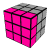
\includegraphics[width=0.1\textwidth]{img/draw_f.png}
    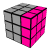
\includegraphics[width=0.1\textwidth]{img/draw_r.png}
    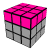
\includegraphics[width=0.1\textwidth]{img/draw_u.png}
    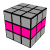
\includegraphics[width=0.1\textwidth]{img/draw_e.png}
    \caption*{\textbf{F}ront \kern 20pt \textbf{R}ight \kern 20pt \textbf{U}pper \kern 16pt  \textbf{E}quator}
\end{figure}

\noindent \textbf{Haltung:} Der Würfel wird so gehalten, dass die \textbf{F}(ront)-Ebene in der linken, die \textbf{R}(ight)-Ebene in der rechten Hand zu liegen kommt.
\end{justify}
\vspace{2mm}

\subsection{Ecken der ersten Seite platzieren}
\begin{justify}
Dieser Schritt ist relativ einfach und erfolgt ohne Anleitung. Er ist abgeschlossen, sobald auf einer Würfelseite die Farben der 4 Ecken mit der Farbe des Mittelteilchens übereinstimmen - in der Abb. weiss markiert:
\end{justify}

\begin{figure}[!htb] 
  \centering
     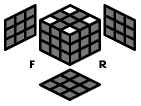
\includegraphics[width=0.20\textwidth]{img/white_corners.png}
\end{figure}

\newpage
\subsection{Ecken der zweiten Seite platzieren}
\begin{justify}
Ist der vorangehende Schritt abgeschlossen, wird der Würfel so um 180\degree gedreht, dass die bearbeitete Seite nach unten zeigt. Dann werden die Ecken der nun nach oben zeigenden Seite, im Bild gelb markiert, gelöst:
\end{justify}

\begin{figure}[!htb] 
  \centering
     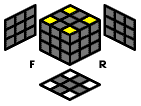
\includegraphics[width=0.20\textwidth]{img/yellow_corners.png}
\end{figure}
\begin{justify}
Um dies zu erreichen muss nun die anzuwendende Zugfolge, abhängig von der Lage der gelb markierten Ecken, ermittelt werden:
\end{justify}

\subsubsection{Buchstabe T-Muster}
\begin{figure}[!htb] 
  \centering
     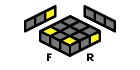
\includegraphics[width=0.20\textwidth]{img/t_pattern.png}
\end{figure}

\centering \textbf{Zugfolge:} R U R' U' F' U' F

\subsubsection{Buchstabe L-Muster}
\begin{figure}[!htb] 
  \centering
     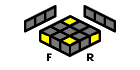
\includegraphics[width=0.20\textwidth]{img/l_pattern.png}
\end{figure}
\centering \textbf{Zugfolge:} F R' F' U' R' U R

\subsubsection{Sune \#1-Muster}
\begin{figure}[!htb] 
  \centering
     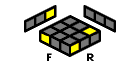
\includegraphics[width=0.20\textwidth]{img/sune_pattern_1.png}
\end{figure}
\centering \textbf{Zugfolge:} R U2 R' U' R U' R'
\newpage

\subsubsection{Sune \#2-Muster}
\begin{figure}[!htb] 
  \centering
     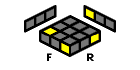
\includegraphics[width=0.20\textwidth]{img/sune_pattern_2.png}
\end{figure}
\centering \textbf{Zugfolge:} R U R' U R U2 R'

\subsubsection{Buchstabe $\pi$-Muster}
\begin{figure}[!htb] 
  \centering
     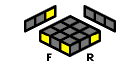
\includegraphics[width=0.20\textwidth]{img/pi_pattern.png}
\end{figure}
\centering \textbf{Zugfolge:} R U R2 F' R2 U R'

\subsubsection{Buchstabe U-Muster}
\begin{figure}[!htb] 
  \centering
     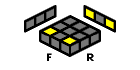
\includegraphics[width=0.20\textwidth]{img/u_pattern.png}
\end{figure}

\centering \textbf{Zugfolge:} R' F' U' F U R

\subsubsection{Buchstabe H-Muster}
\begin{figure}[!htb] 
  \centering
     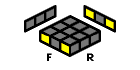
\includegraphics[width=0.20\textwidth]{img/h_pattern.png}
\end{figure}
\centering \textbf{Zugfolge:} R2 U2 R' U2 R2

\subsection{Alle Ecken richtig \newline orientieren}
\begin{justify}
In diesem Schritt werden alle 8 Ecken durch Anwenden einer einzigen Zugfolge richtig ausgerichtet. Um zu ermitteln, welche Zugfolge anzuwenden ist, müssen in der obersten und untersten Schicht die paarweise gleichfarbigen Eckenpaare gezählt werden. 
\end{justify}

\newpage
\subsubsection{Kein Eckenpaar gleichfarbig}
\begin{figure}[!htb] 
  \centering
     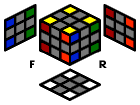
\includegraphics[width=0.20\textwidth]{img/orient-0-solved.png}
\end{figure}
\centering \textbf{Zugfolge:} R2 F2 R2
        
\subsubsection{Eckenpaar hinten unten\newline gleichfarbig}
\begin{figure}[!htb] 
  \centering
     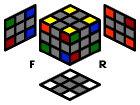
\includegraphics[width=0.20\textwidth]{img/orient-db-solved.png}
\end{figure}
\centering \textbf{Zugfolge:} R U' F U2 F' U R'

\subsubsection{Zwei Eckenpaare hinten\newline gleichfarbig}
\begin{figure}[!htb] 
  \centering
     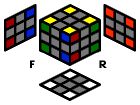
\includegraphics[width=0.20\textwidth]{img/orient-db-ub-solved.png}
\end{figure}
\centering \textbf{Zugfolge:} R2 U F2 U2 R2 U R2 

\subsubsection{Vier Eckenpaare unten\newline gleichfarbig}
\begin{figure}[!htb] 
  \centering
     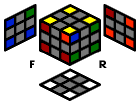
\includegraphics[width=0.20\textwidth]{img/orient-4d-solved.png}
\end{figure}
\centering \textbf{Zugfolge:} F2 U' R U' R' U F2 U R U R' 

\newpage
\subsubsection{Fünf Eckenpaare unten und oben hinten gleichfarbig}
\begin{figure}[!htb] 
  \centering
     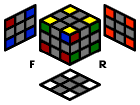
\includegraphics[width=0.20\textwidth]{img/orient-uf-not-solved.png}
\end{figure}
\centering \textbf{Zugfolge:} R U' R F2 R' U R F2 R2 
        
\vspace{6mm}
\section{2) Kanten der U/D-Ebenen orientieren}
\begin{justify}
Nachdem alle 8 Ecken korrekt orientiert sind, werden die Kanten - d.h. jene Teilchen mit zwei Stickern - der unteren und oberen Ebene korrekt platziert und orientiert. 
\end{justify}
\begin{figure}[!htb] 
  \centering
     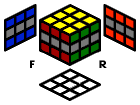
\includegraphics[width=0.20\textwidth]{img/set2solved.png}
\end{figure}

\subsection{Kanten platzieren und\newline orientieren}
\begin{justify}
Die Kantenteilchen werden jetzt Kante für Kante mit den nachfolgenden Zugfolgen platziert und orientiert. Man löst so zuerst die untere Ebene - bis auf eine Kante:
\begin{figure}[!htb] 
  \centering
     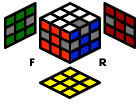
\includegraphics[width=0.20\textwidth]{img/single-gap-unsolved.png}
\end{figure}
\end{justify}

\newpage
\subsubsection{Kante von hinten nach vorne unten}
\begin{figure}[!htb] 
  \centering
     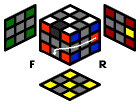
\includegraphics[width=0.20\textwidth]{img/hinten-rechts-vorne-unten.png}
\end{figure}
\centering \textbf{Zugfolge:} F' E F

\subsubsection{Kante von hinten nach vorne unten\newline gedreht}
\begin{figure}[!htb] 
  \centering
     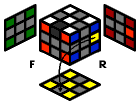
\includegraphics[width=0.20\textwidth]{img/hinten-rechts-vorne-unten-2.png}
\end{figure}
\centering \textbf{Zugfolge:} F E2 F'

\subsubsection{Kante von oben nach unten}
\begin{figure}[!htb] 
  \centering
     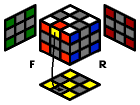
\includegraphics[width=0.20\textwidth]{img/oben-nach-unten.png}
\end{figure}
\centering \textbf{Zugfolge:} F E F'

\subsubsection{Kante von oben nach unten\newline gedreht}
\begin{figure}[!htb] 
  \centering
     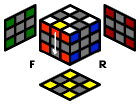
\includegraphics[width=0.20\textwidth]{img/oben-nach-unten2.png}
\end{figure}
\centering \textbf{Zugfolge:} F E' F2 E F

\newpage
\subsubsection{Kante vorne unten kippen}
\begin{figure}[!htb] 
  \centering
     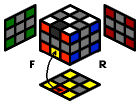
\includegraphics[width=0.20\textwidth]{img/oben-unten-nach-unten-twist.png}
\end{figure}
\centering{\textbf{Zugfolge:} F' E' F2 E2 F'}

\begin{justify}
Wurden drei beliebige Kanten in der unteren Ebene korrekt platziert und orientiert, wird die Unterseite nach oben gedreht und die vier Kantenteilchen der jetzt nach unten zeigenden Ebene platziert und orientiert.\\

\indent Dabei ist zu beachten, dass die Lücke - d.h. das ungelöste Kante der oberen Ebene - immer gegenüber dem zu lösenden Kantenteilchens der Unterseite positioniert wird. Die Lücke ist in den Bildern grau markiert.
\end{justify}

\subsection{Letzte Kante lösen}
\begin{justify}
Jetzt muss noch die letzte Kante der U(pper)-Ebene gelöst werden. Je nach  Situation kann eine der nachfolgenden 3 Zugfolgen eingesetzt werden. Allenfalls muss vorgängig noch die E(quator)-Ebene ausgerichtet werden, damit eine der nachfolgenden Konstellationen erkennbar werden.
\end{justify}
\subsubsection{Kante kippen}
\begin{figure}[!htb] 
  \centering
     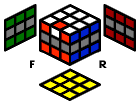
\includegraphics[width=0.20\textwidth]{img/swap_cant.png}
\end{figure}
\centering{\textbf{Zugfolge:} F E' F E' F E' F}

\newpage
\subsubsection{Kante von hinten rechts nach \newline vorne oben}
\begin{figure}[!htb] 
  \centering
     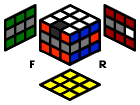
\includegraphics[width=0.20\textwidth]{img/stopf_easy.png}
\end{figure}
\centering{\textbf{Zugfolge:} F E' F' E F E F'}

\subsubsection{Kante von hinten rechts nach \newline vorne oben gedreht}
\begin{figure}[!htb] 
  \centering
     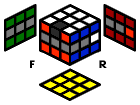
\includegraphics[width=0.20\textwidth]{img/stopf_hard.png}
\end{figure}
\centering{\textbf{Zugfolge:} F E' F2 E' F}

\section{3) M-Ebene lösen}
\begin{justify}
Zum Abschluss muss nun noch die verbleibende mittlere Ebene gelöst werden. Dabei kommen folgende drei Züge zum Einsatz:\\

\noindent \textbf{Züge:} \textbf{M}=middle, \textbf{U}=upper, \textbf{S}=standing; die Appostrophe kennzeichnen Drehungen im Gegenuhrzeigersinn bei senkrechtem Blick auf die jeweilige Ebene.

\begin{figure}[!htb] 
    \centering
    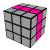
\includegraphics[width=0.1\textwidth]{img/draw_m.png}
    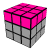
\includegraphics[width=0.1\textwidth]{img/draw_u.png}
    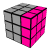
\includegraphics[width=0.1\textwidth]{img/draw_r.png}
    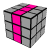
\includegraphics[width=0.1\textwidth]{img/draw_s.png}
    \caption*{\textbf{M}iddle \kern 17pt \textbf{U}pper \kern 13pt \textbf{F}ront \kern 17pt \textbf{S}tanding}
\end{figure}

\noindent \textbf{Haltung:} Der Würfel wird so gehalten, dass die \textbf{L}(eft)-Ebene in der linken und die \textbf{R}(ight)-Ebene in der rechten Hand zu liegen kommt.

\begin{figure}[!htb] 
  \centering
     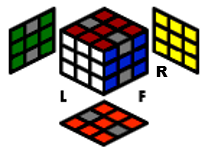
\includegraphics[width=0.20\textwidth]{img/center_demo.png}
\end{figure}
\end{justify}

\subsection{Kanten platzieren}
\begin{justify}
In diesem Schritt werden die Kanten der M-Ebene platziert, bevor sie dann im letzten Schritt noch korrekt orientiert werden. Es kann eine der nachfolgenden drei Situationen vorliegen.
\end{justify}

\subsubsection{Kanten permutieren}
\begin{justify}
Diese Zugfolge ist dann zu wählen, wenn die einzig korrekte Kante der mittleren Schicht hinten unten liegt und die vorne oben liegende Kante nach vorne unten wandern soll:
\end{justify}
\begin{figure}[!htb] 
  \centering
     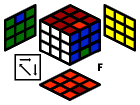
\includegraphics[width=0.20\textwidth]{img/middle-permutate.png}
\end{figure}
\centering{\textbf{Zugfolge:} M U2 M' U2}

\subsubsection{Kanten horizontal tauschen}
\begin{justify}
Diese Zugfolge ist dann zu wählen, wenn die Kantenteilchen der Mittelschicht horizontal ausgetauscht werden sollen.  
\end{justify}
\begin{figure}[!htb] 
  \centering
     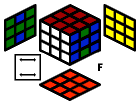
\includegraphics[width=0.20\textwidth]{img/middle-translate.png}
\end{figure}
\centering{\textbf{Zugfolge:} M2 U2 M2 U2}

\subsubsection{Kanten diagonal tauschen}
\begin{justify}
Diese Zugfolge ist dann zu wählen, wenn die Kantenteilchen der Mittelschicht diagonal ausgetauscht werden sollen.
\end{justify}
\begin{figure}[!htb] 
  \centering
     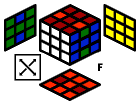
\includegraphics[width=0.20\textwidth]{img/middle-crossover.png}
\end{figure}
\centering{\textbf{Zugfolge:} M S2 M S2}

\newpage
\subsection{Kanten orientieren}
\begin{justify}
Nun sind alle Kanten der M-Ebene dort, wo sie sein sollen, können aber noch gekippt sein. In diesem letzten Schritt werden die letzten Kanten der M-Ebene noch korrrekt orientiert. Es kann eine von drei Situationen vorliegen.
\end{justify}

\subsubsection{Obere Kanten der Mittelschicht kippen}
\begin{justify}
Diese Zugfolge ist dann zu wählen, wenn die Kantenteilchen der Mittelschicht diagonal ausgetauscht werden sollen.
\end{justify}
\begin{figure}[!htb] 
  \centering
     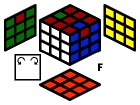
\includegraphics[width=0.20\textwidth]{img/middle-topswap.png}
\end{figure}
\centering{\textbf{Zugfolge:} M U M U M U2 M' U M' U M' U2} 

\subsubsection{Diagonal gegenüberliegende Kanten kippen}
\begin{justify}
Liegen 2 diagonal gegenüber liegende gekippte Kantenteilchen vor, so kann der Würfel durch eine 180\degree Drehung der Front- oder Rückseite auf dasselbe Problem zurückgeführt werden, so dass dann wieder die obige Zugfolge zum Ziel führt. Abschliessend ist dann nur noch diese 180\degree Drehung der Front- / Rückseite rückgängig zu machen und der Würfel ist gelöst.
\end{justify}

\subsubsection{Alle Kanten der Mittelschicht \newline kippen}
\begin{justify}
Relativ selten kommt es vor, dass alle 4 Eckpunkte der Mittelschicht gekippt werden müssen. In diesen Fällen führt untenstehende Zugfolge zum Ziel:
\end{justify}
\begin{figure}[!htb] 
  \centering
     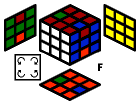
\includegraphics[width=0.20\textwidth]{img/middle-allswap.png}
\end{figure}
\centering{\textbf{Zugfolge:} F' L' F M U M U M U M U F' L F} 
            

% End document
\end{document}
